% 
% sample.tex
%
%   This is LaTeX template to get you started
%   making problem-set solutions
%
 
\documentclass[11pt]{article}
\usepackage{amsmath}
\usepackage{algorithm2e}
\usepackage{graphicx}
\usepackage{hyperref}

\setlength{\oddsidemargin}{0in}
\setlength{\evensidemargin}{0in}
\setlength{\textheight}{9in}
\setlength{\textwidth}{6.5in}
\setlength{\topmargin}{-0.5in}

% Sample macros -- how you define new commands
% My own set of frequently-used macros has grown to many hundreds of lines
\newcommand{\Adv}{{\mathbf{Adv}}}       
\newcommand{\prp}{{\mathrm{prp}}}                  % How to define new commands 
\newcommand{\calK}{{\cal K}}
\newcommand{\outputs}{{\Rightarrow}}                
\newcommand{\getsr}{{\:\stackrel{{\scriptscriptstyle\hspace{0.2em}\$}}{\leftarrow}\:}}
\newcommand{\andthen}{{\::\;\;}}    % \, \: \; for thinspace, medspace, thickspace
\newcommand{\Rand}[1]{{\mathrm{Rand}[{#1}]}}       % A command with one argument
\newcommand{\Perm}[1]{{\mathrm{Perm}[{#1}]}}       
\newcommand{\Randd}[2]{{\mathrm{Rand}[{#1},{#2}]}} % and with two arguments

\newcommand{\sym}[1]{{\tt \bf {#1}}}
\newcommand{\abs}[1]{{$\left|{#1}\right|$}}

%%%%%%%%%%%%%%%%%%%%%%%%%%%%%%%%%%%%%%%%%%%%%%%%%%%%%%%%%%%%%%%%%%%%%%%%%%%
\title{\bf The Turing Machine Program\\[2ex] 
       \rm\Large Assignment 1.1, CS9163 - Application Security}
\author{Bowen Yu, 0487810}
\date{\today}


\begin{document}
\maketitle
\large

%%%%%%%%%%%%%%%%%%%%%%%%%%%%%%%%%%%%%%%%%%%%%%%%%%%%%%%%
\section{Overview}
The Turing Machine (TM) is implemented using the sandbox's coding language. It uses an array to simulate the Turing Machine tape and reads a special type of data that gives the Turing Machine's symbol collection, deterministic finite automaton (DFA), and the tape contents. The program of the Turing Machine is given in the file {\tt tm\_prog}. It requires a data file to run. The TM data describes a TM using integer encoding to meet the sandbox's requirement. Details of how to write a data file in given in Section~\ref{sec:data}. An example data file is provided as {\tt tm\_data} (Section~\ref{sec:example}), which defines a Turing Machine that computes the Bitwise-OR operation.

\section{Data Specification}
\label{sec:data}
The first part of the data contains one integer {\tt K}, specifying the size of the symbol collection. Indeed, there are {\tt K+1} symbols as the TM automatically includes a void symbol {\tt \#}. The void symbol is encoded as integer 0. The other {\tt K} symbols are encoded as integers from 1 to {\tt K}.\\\\
The second part of the data specifies the DFA. It begins with an integer {\tt N}, the number of states. States are numbered from 0 to {\tt N-1}. For each state, there shall be a line describing its type (Left or Right), and its number of outward transitions {\tt L}. Type Left is encoded as 0 while Type Right is encoded as 1. Following this line shall be {\tt L} lines, each of which has three integers representing the accept symbol, the write symbol and the transition state (all encoded using integers as described above).\\\\
The third part of the data gives the start and halt states of the TM using two integers.\\\\
The fourth part of the data describes the original TM tape. The first line has two integers, the number of tape cells {\tt C} that originally contain data and the initial cell. Then follows a line with {\tt C} integers, describing the cell data from left to right using the integer symbol encoding.\\\\
The final part of the data provides the expected TM output tape range. That is, after the TM halts, the system will output the data in the cells specified here. This part shall begin with an integer {\tt S}, the number of range segments. Then each segment is given as a pair of integers giving the beginning location of the segment and the length of the segment, e.g. {\tt 0 4} represents cell location {\tt 0, 1, 2, 3}. \\

\section{Example Data}
\label{sec:example}
The {\tt tm\_data} file contains a TM data example that performs Bitwise-OR on two binary numbers.\\\\
The DFA of this TM is shown as the picture below, which is a snapshot of a Java TM Simulator at \url{http://introcs.cs.princeton.edu/java/74turing}. The details of the graph representations in the picture can also be found on this website. \\
\\
Basically, the graph describes the transitions between different TM states. On a state, the TM reads in the symbol on the current tape cell and match it with any outward edges of the current state (symbols to the left of the colons). If a matching is found, the TM write the pairing symbol (to the right of the colon) to the current cell and jump to the target state along the edge. Then it moves the tape head left or right based on the target state's type. The TM halts when a halt state is reached.\\
\begin{figure}[hp]
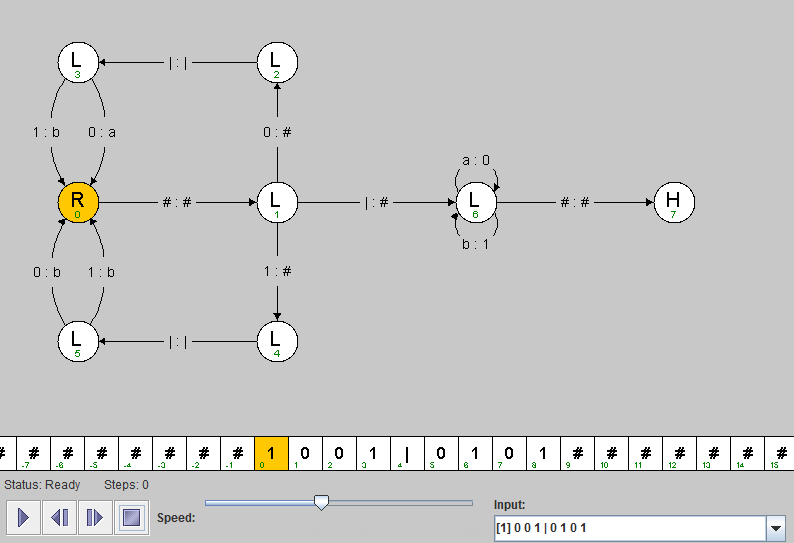
\includegraphics[width=\textwidth]{tm_bitwise_or}
\end{figure}
\\
The example data describes this TM using the format specified in Section~\ref{sec:data}. The integer encoding of symbols are: {\tt \#} as 0, {\tt 0} as 1, {\tt 1} as 2, {\tt a} as 3, {\tt b} as 4. At the end of the data, it specifies one output segment which is the four cells with locations {\tt 0-3}, as the result of the Bitwise-OR TM. The TM tape originally has two binary numbers 1001 and 0101. The Bitwise-OR result is 1101, which can be verified as the example program outputs 2212 in the end (the integer encoding of binary number 1101).

\section{TM Program}
The program of the TM is given as the file {\tt tm\_prog}. \\\\
There would be a lot of tedious details to explain the whole TM program. But the logic is simple. The program allocates a large enough array to simulate the TM tape, and a predefined set of arrays to store the state transition graph. It reads the data in and start the TM with the starting location of tape head, and the starting state specified in the data. When a symbol needs to be read/written from/to the tape, the TM program just reads/writes it from/to the tape array. When changing states/tape head, the TM program just changes the state/tape-head index so as to locate a state in the array. To simulate the infinite tape, the starting index is moved to the center of the array in order to make sure that both left and right side have enough expansion space. However, it may be possible that the TM runs far away from this limited-length simulated tape. In this case, the program will report error as there is insufficient memory to support the TM execution. The array size can be set in the first few lines of the program (like macros) and can be changed based on different TM tasks. But the total size must not exceed the memory limit of the sandbox. \\
\\
Necessary comments have been added to the program file to help better understanding. 

\section{Error Handling}
Note that the TM program is not responsible for any data errors. If you are going to write a TM data file, you need to make sure that the data file follows the TM data format described above. You also need to ensure the DFA in your data is valid. However, the sandbox is responsible for handling any errors a misbehaving program may cause. For example, if the array index the TM is trying to access is out of range, the sandbox will detect it and stop the TM program.
\end{document}